%% SECTION HEADER /////////////////////////////////////////////////////////////////////////////////////
\section{Damage indices}
\label{sec:di}

%% SECTION CONTENT ////////////////////////////////////////////////////////////////////////////////////
In the dissertation, six damage indices, considered to be the most effective \cite{torkamani2014novel, moix2016damage}, were analysed based on the signal envelope in the time-domain registered by the sensor.
All of them were considered in three variants: (i) the full-length of the signal, (ii) the first wave packet of the \ac{s0}, (iii) the first wave packet of the \ac{a0}.
The analysis considered signals at 50, 100 and 150 \unit{\kHz}, with the last frequency excluded for the \ac{a0}, because, as indicated in Section~\ref{sec:resuls_pzt}, this mode was masked by reflections of the \ac{s0}.
The wave packets were extracted by windowing the full-length signals with a flattened Gaussian window in the form
\begin{eqnarray}
	g(t)= \mathrm{exp}\left(-\left(\frac{t-t_0}{w_g}\right) ^{s}\right),
	\label{eq:psi_g}
\end{eqnarray}
\nomtypeD[gt]{\(g(t)\)}{Gaussian window}{}%
where \(t_0\) and \(w_g=0.5N_c/f_c\) are the center point and the half-width of the window, respectively, and \(s\) determines the slope of the window. Figure~\ref{fig:windows} depicts the usage of the window.
\begin{figure}[!tbh]
	\begin{center}
		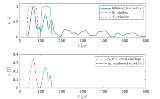
\includegraphics[width=0.95\textwidth]{Chapter_7/windows}
	\end{center}
	\caption{The signal envelop and the Gaussian windows}
	\label{fig:windows}
\end{figure}
\pagebreak

The following time-domain indices were taken into consideration: \ac{p2p}, \ac{saps}, \ac{sapr}, \acf{rmsd}, \ac{eng} and \ac{cc}.
Definitions of these metrics are as follows:
\begin{eqnarray}
	\mathrm{P2P} & = & \mathrm{max}(e_H) - \mathrm{max}(e_D),\\
	\mathrm{SAPS} & = & 1 - \left[\frac{\mathrm{max}(e_H)-\mathrm{max}(e_D)}{\mathrm{max}(e_H)}\right]^2,\\
	\mathrm{SAPR} & = & \frac{\mathrm{max}(e_H)}{\mathrm{max}(e_D)},\\
	\mathrm{RMSD} & = & 1 - \sqrt{\frac{\sum_{i=1}^{l}\left(e_D-e_H\right)^2}	{\sum_{i=1}^{l}e_H^2}},\\
	\mathrm{ENG} & = & 1 -  \frac{\sum_{i=1}^{l}{e_D^2}-\sum_{i=1}^{l}{e_H^2}}{\sum_{i=1}^{l}{e_H^2}},\\
	\mathrm{CC} & = & \frac{l\sum_{i=1}^{l}e_De_H-\sum_{i=1}^{l}e_D\sum_{i=1}^{l}e_H}{\sqrt{l\sum_{i=1}^{l}e_D^2-\left[\sum_{i=1}^{l}e_D\right]^2}\sqrt{l\sum_{i=1}^{l}e_H^2-\left[\sum_{i=1}^{l}e_H\right]^2}},
\end{eqnarray}
where \(e_H\) and \(e_D\) are the envelope of the signal registered by the sensor for the healthy and damaged state of the specimen, respectively, \(l\) is the length of the signal, and max\((e)\) is maximum value of the signal envelope.
The \ac{p2p}, \ac{saps}, \ac{sapr} are based on the difference between amplitudes of the monitored and the baseline state.
The \ac{rmsd} measures the error between baseline and damaged, \ac{eng} compares the difference of the sensor responses energy and \ac{cc} is the index based on Pearson correlation coefficient.

\begin{figure}[!tbh]
	\begin{center}
		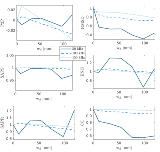
\includegraphics[width=0.95\textwidth]{Chapter_7/DI_full_full}
	\end{center}
	\caption{The \aclp{di} obtained with the \acl{fcgm} based on the full-length signals}
	\label{fig:DI_full_full}
\end{figure}
\begin{figure}[!tbh]
	\begin{center}
		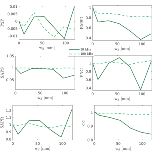
\includegraphics[width=0.95\textwidth]{Chapter_7/DI_full_A0}
	\end{center}
	\caption{The \aclp{di} obtained with the \acl{fcgm} based on the \acs{a0} windowed signal}
	\label{fig:DI_full_A0}
\end{figure}
\begin{figure}[!tbh]
	\begin{center}
		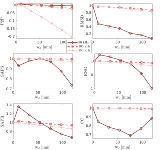
\includegraphics[width=0.95\textwidth]{Chapter_7/DI_full_S0}
	\end{center}
	\caption{The \aclp{di} obtained with the \acl{fcgm} based on the \acs{s0} windowed signal}
	\label{fig:DI_full_S0}
\end{figure}

The \acp{di} based on full-length signals derived from simulations with the \ac{fcgm} are presented in Figure~\ref{fig:DI_full_full}.
The damage was modelled by removing the core cells in the damage area.
Noticeably, all the \acp{di} for 50 \unit{\kHz} are not monotonous.
This is due to the fact that a low-frequency wave (up to 100 \unit{\kHz}, according to work of Tian et al. \cite{tian2015wavenumber}), propagated through the entire thickness of \ac{hsc}.
Therefore, in the analysis of damage size, not only the phenomenon of wave leakage was relevant, but also the reflection from cell walls.  
The high-frequency wave propagated mainly through the skin of the panel, so changes in the signal recorded by the sensor in the damaged sample were mainly caused by the wave leakage effect.

The \acp{di} based on the windowed signals are shown in Figures~\ref{fig:DI_full_A0} and \ref{fig:DI_full_S0} for the \ac{a0} and \ac{s0} window, respectively.
It should be mentioned that \acp{di} for 150 \unit{\kHz} were omitted in Figure~\ref{fig:DI_full_A0}, due to the masking of this mode by the \ac{s0} reflections.
The characteristics of the \ac{s0}-based indices are consistent with the related indices determined for the full-length signals, although for most indices, their values are less than those of full-length signals.
The \ac{s0}-based \acp{di} values are also less than the \ac{a0}-based signals, except the \ac{rmsd} at 50 \unit{kHz}.
It is because dominant displacements of the \ac{s0} are in-plane of the skin, so less portion of the wave energy leak into the core through the healthy region.
In the case of the full-length response, the \ac{a0} was registered, which is more susceptible to damage in the form of disbonds or delamination since its main displacements are out-of-plane.

Accordingly, the following indicators were selected for further consideration: \ac{p2p} and \ac{sapr} at 150 \unit{kHz} (see Figures \ref{fig:DI_P2P} and \ref{fig:DI_SAPR}), \ac{rmsd} and \ac{cc}, all in the case of full-length and at 100 and 150 \unit{\kHz} (see Figures \ref{fig:DI_RMSD_full} and \ref{fig:DI_CC}), and \ac{rmsd} at 50 \unit{kHz} \ac{s0}-based signals (see Figure \ref{fig:DI_RMSD_S0}).
Selected indicators were also determined for damage modeled by removing interface elements. Then, they were compered with the indices obtained for the \ac{hcgm}.

\begin{figure}[!tbh]
	\begin{center}
		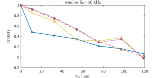
\includegraphics[width=0.95\textwidth]{Chapter_7/DI_P2P}
	\end{center}
	\caption{Comparison of the selected \acfp{p2p} based on full-length signals for the various models of the core and damage: the \acf{fcgm} with removed core cells (solid line), the \ac{fcgm} with removed interface elements (dashed line), the \acf{hcgm} with removed core cells (dash-dot line), the \ac{hcgm} with removed interface elements(dotted line)}
	\label{fig:DI_P2P}
\end{figure}

\begin{figure}[!tbh]
	\begin{center}
		\includegraphics[width=0.95\textwidth]{Chapter_7/DI_SAPR}
	\end{center}
	\caption{Comparison of the selected \acfp{sapr} based on full-length signals for the various models of the core and damage: the \acf{fcgm} with removed core cells (solid line), the \ac{fcgm} with removed interface elements (dashed line), the \acf{hcgm} with removed core cells (dash-dot line), the \ac{hcgm} with removed interface elements (dotted line)}
	\label{fig:DI_SAPR}
\end{figure}
It can be noticed that \ac{p2p} and \ac{sapr} differ significantly in terms of the core model used. Both indexes for the \ac{fcgm} are continuously decreasing, while for the \ac{hcgm}, the values are almost constant in the whole range of damage.
In addition, the damage model has little effect only for the \ac{fcgm}.
The values for all cases are consistent for the \ac{rmsd} based on the \ac{s0} window.
Only the \ac{fcgm} for the two smallest damage scenarios deviates from the other models.
For the \ac{rmsd} and the \ac{cc} based on full-length signals, the results are comparable for the all models, except the values for the \ac{hcgm} at 100 \unit{kHz} are more significant than the \ac{fcgm}.
\begin{figure}[!tbh]
	\begin{center}
		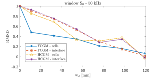
\includegraphics[width=0.95\textwidth]{Chapter_7/DI_RMSD_S0}
	\end{center}
	\caption{Comparison of the selected \acfp{rmsd} based on \ac{s0} windowed signals for the various models of the core and damage: the \acf{fcgm} with removed core cells (solid line), the \ac{fcgm} with removed interface elements (dashed line), the \acf{hcgm} with removed core cells (dash-dot line), the \ac{hcgm} with removed interface elements (dotted line)}
	\label{fig:DI_RMSD_S0}
\end{figure}

\begin{figure}[!tbh]
	\begin{center}
		\includegraphics[width=0.95\textwidth]{Chapter_7/DI_RMSD_full}
	\end{center}
	\caption{Comparison of the selected \acfp{rmsd} based on full-length signals for the various models of the core and damage: the \acf{fcgm} with removed core cells (solid line), the \ac{fcgm} with removed interface elements (dashed line), the \acf{hcgm} with removed core cells (dash-dot line), the \ac{hcgm} with removed interface elements (dotted line)}
	\label{fig:DI_RMSD_full}
\end{figure}

\begin{figure}[!bh]
	\begin{center}
		\includegraphics[width=0.95\textwidth]{Chapter_7/DI_CC_full}
	\end{center}
	\caption{Comparison of the selected \acfp{cc} based on full-length signals for the various models of the core and damage: the \acf{fcgm} with removed core cells (solid line), the \ac{fcgm} with removed interface elements (dashed line), line the \acf{hcgm} with removed core cells (dash-dot), the \ac{hcgm} with removed interface elements (dotted line)}
	\label{fig:DI_CC}
\end{figure}